\chapter{Mean and Variance}

% ------------------------------------------------------ %
\section{Summarizing Data on Random Variables}
Often times, listing out all of the outcomes of a sample is not a very helpful way of communicating the information obtained from the sample. A common, more helpful way to present the data of a sample is a \textbf{frequency distribution}. A frequency distribution gives the number of times each value of a random variable $X$ occurred.
\begin{center}
\begin{tabular}{ |c|c|c|c| } 
\hline
$X$ & Frequency Count & Frequency \\
\hline
1 & \StrokeTwo & 2 \\ 
2 & \StrokeFive\StrokeOne & 6 \\ 
3 & \StrokeFive & 5 \\
4 & \StrokeThree & 3 \\
\hline
\end{tabular}
\end{center}
We could also draw a \textbf{frequency histogram} of these frequencies.
\begin{center}
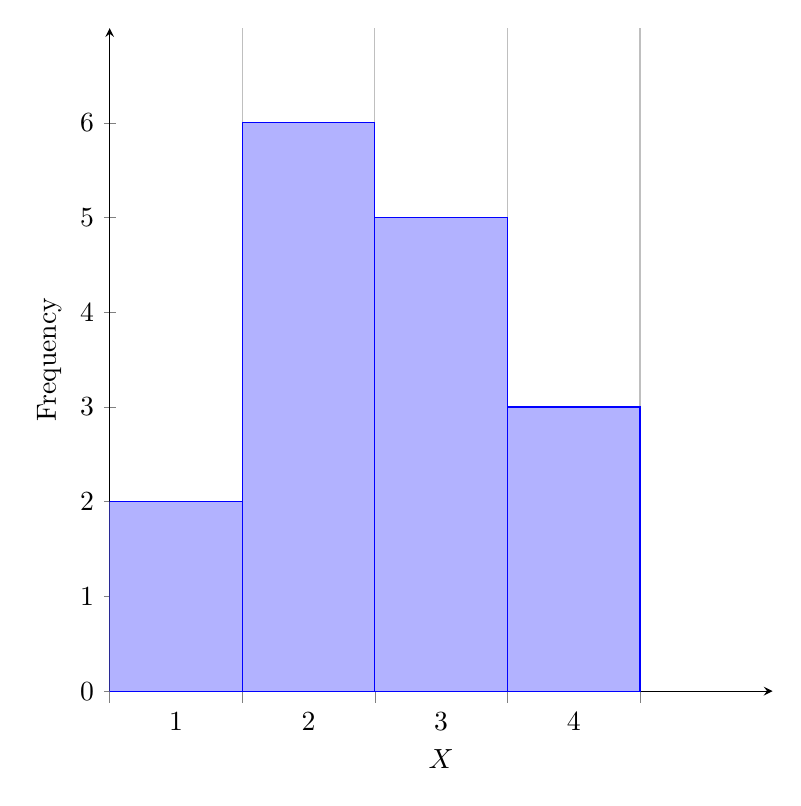
\begin{tikzpicture}
\begin{axis}[
	ylabel=Frequency,xlabel=$X$,
	axis lines=left,
	ymax=7,
	xmax=5,
	ybar interval=1,
	ytick = {0,...,6},
	width=10cm,height=10cm,
]
\addplot
	coordinates {(4,3) (3,5) (2,6) (1,2) (0,0)};
\end{axis}
\end{tikzpicture}
\end{center}
Frequency distributions are good summaries of data because they show the variability in the observed outcomes clearly. Another way to summarize results are single-number summaries such as the following:
\bigskip\par
The \textbf{mean} of a sample of outcomes is the average value of the outcomes. It is the sum of the outcomes divide by the total number of outcomes. The mean of $n$ outcomes, $x_1,\ldots,x_n$, for a random variable $X$ is
\[
    \sum_{i = 0}^{n} \frac{x_i}{n} = \frac{x_1,\ldots,x_n}{n}
\]
\bigskip\par
The \textbf{median} of a sample is an outcome such that half the outcomes are before it and half the outcomes are after it when the outcomes are arranged in numerical order.
\bigskip\par
The \textbf{mode} of a sample is the outcome that occurs most frequently. There can be multiple equal modes in a sample.
\bigskip\par
\begin{example}
A fisherman records the weight of each fish he catches for a week. These are his results. Each value represents the weight, in pounds, of a fish he caught.
\[
    \{\, 20,23,19,27,17,22,18,15,23,25,18,23,29 \,\}
\]
A frequency distribution of the sample above is
\begin{center}
\begin{tabular}{ |c|c|c|c| } 
\hline
$X$ & Frequency Count & Frequency \\
\hline
15 & \StrokeOne & 1 \\ 
17 & \StrokeOne & 1 \\ 
18 & \StrokeTwo & 2 \\ 
19 & \StrokeOne & 1 \\
20 & \StrokeOne & 1 \\
22 & \StrokeOne & 1 \\ 
23 & \StrokeThree & 3 \\ 
25 & \StrokeOne & 1 \\ 
27 & \StrokeOne & 1 \\
29 & \StrokeOne & 1 \\
\hline
\end{tabular}
\end{center}
And the following is a frequency histogram
\begin{center}
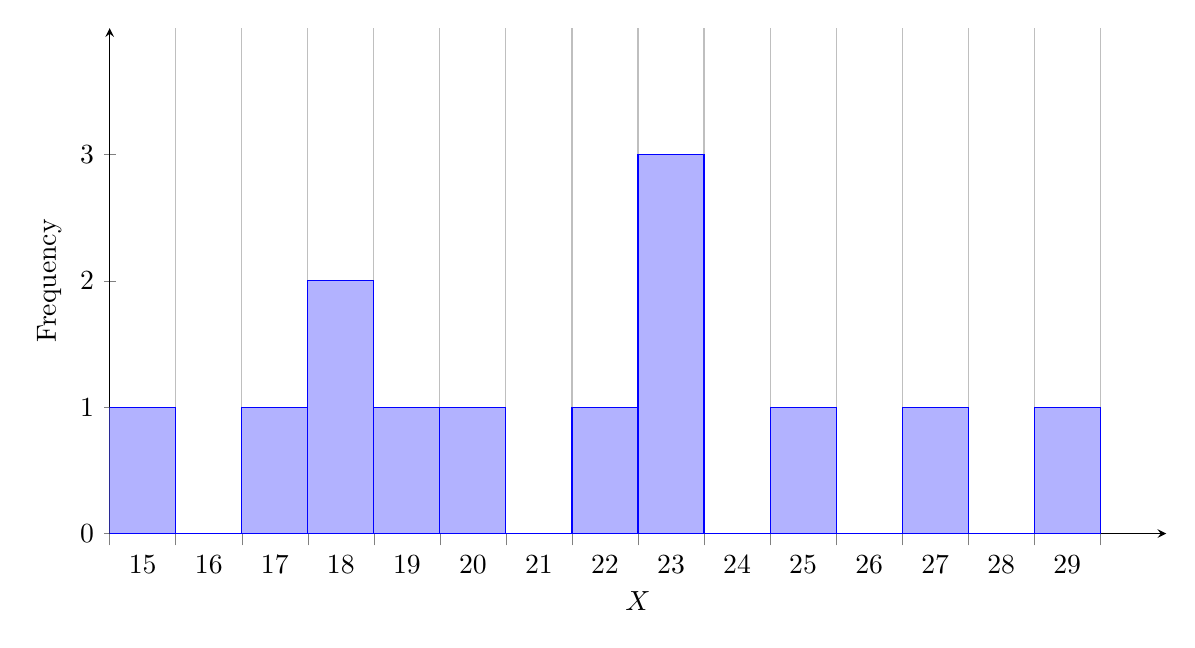
\begin{tikzpicture}
\begin{axis}[
	ylabel=Frequency,xlabel=$X$,
	axis lines=left,
	ymax=4,	
	xmin=14,
	xmax=30,
	ybar interval=1,
	ytick = {0,1,2,3},
	width=15cm,height=8cm,
]
\addplot
	coordinates {(29,1) (28,0) (27,1) (26,0) (25,1) (24,0) (23,3) (22,1) (21,0) (20,1) (19,1) (18,2) (17,1) (16,0) (15,1) (14,0)};
\end{axis}
\end{tikzpicture}
\end{center}
The mean weight of sample of fishes is
\[
    \frac{20+23+19+27+22+18+15+23+18+23+29}{13} = \frac{237}{13} \approx 18.231
\]
The median weight of the sample of fishes is found by rearranging the sample into numerical order and selecting the middle outcome. The median is 22.
\[
    15,18,18,19,20,\underuparrow{22},23,23,23,27,29
\]
The mode is the weight that occurs most frequently. It corresponds to tallest bar on the histogram. 23lbs occurs the most (3 times) so it is the median.
\end{example}

% ------------------------------------------------------ %
\section{Expected Value of a Random Variable}
The expected value of a random variable $X$ with a range of $A$ and a probability function $f(x)$, is given by
\[
    E(X) = \mean = \sum_{x \in A} xf(x)
\]
\begin{info}
Note that in order to calculate the expected value of a random variable $X$, we often need to know the distribution, and hence the probability function, of $X$.
\end{info}
\begin{theory}{Derivation of the Expected Value}
Suppose we have a frequency distribution of a random variable X, as shown below:
\begin{center}
\begin{tabular}{ |c|c|c|c| } 
\hline
$X$ & Frequency Count & Frequency \\
\hline
5 & \StrokeFive\StrokeFive & 10 \\ 
10 & \StrokeFive\StrokeTwo & 7 \\ 
25 & \StrokeFive\StrokeFive\StrokeThree & 13 \\
100 & \StrokeFour & 4 \\
200 & \StrokeTwo & 1 \\ 
\hline
\end{tabular}
\end{center}
As we learnt in the previous section, we can calculate the mean as
\begin{align*}
    &\frac{(5\times10) + (10\times2) + (25\times13) + (100\times4) + (200\times1)}{30} \\
    &= (5)\left(\frac{10}{30}\right) + (10)\left(\frac{7}{30}\right) + (25)\left(\frac{13}{30}\right) + (100)\left(\frac{4}{30}\right) + (200)\left(\frac{1}{30}\right) \\
    \text{($A$ is the range  of $X$) }
    &=\sum_{x \in A} x \times \text{the fraction of times $x$ occurs}
\end{align*}
Now suppose we know the probability function of $X$ is as follows
\renewcommand{\arraystretch}{1.5}
\begin{center}
\begin{tabular}{ c|c c c c c } 
$x$ & 5 & 10 & 25 & 100 & 200 \\
\hline
$f(x)$ & $\frac{1}{3}$ & $\frac{7}{30}$ & $\frac{13}{30}$ & $\frac{2}{15}$ & $\frac{1}{30}$ \\
\end{tabular}
\end{center}
Using the relative frequency definition of probability, we know that if we observed a very large number of outcomes, the fraction of times $X=x$ occurs (relative frequency of $x$) is $f(x)$. \\ Thus, \textit{in theory}, we would expect the mean of a sample of infinitely many outcomes to be
\[
    (5)\left(\frac{1}{3}\right) + (10)\left(\frac{7}{30}\right) + (25)\left(\frac{13}{30}\right) + (100)\left(\frac{2}{15}\right) + (200)\left(\frac{1}{30}\right) \approx 33.167
\]
This theoretical mean is denoted by $\mu$ or $E(X)$, and is known as the expected value of $X$.
\end{theory}
\begin{example}
A slots machine in a casino costs \$5 to play. It has probabilities of 0.5 to pay out \$2, 0.2 to pay out \$5, a 0.1 to pay out \$10 and otherwise does not pay out anything. Let the random variable $X$ be the amount of money (in dollars) the machine pays out in one play, and $Y$ be the amount of money won or lost in one play. Find $E(X)$ and $E(Y)$.
\[
    E(X) = (0)(0.2) + (2)(0.5) + (5)(0.2) + (10)(0.1) = 3
\]
\[
    E(Y) = (-5)(0.2) + (-3)(0.5) + (0)(0.2) + (5)(0.1) = -2
\]
Note that $E(Y) = E(X - 5) = E(X) - 5$
\end{example}

\begin{example}
A nightclub lets groups of up to 6 people enter at reduced fees. A randomly selected group in the nightclub's line has the following probabilities for its size and cost of entry:
\begin{center}
\begin{tabular}{ |c|c|c| } 
\hline
Size of Group (X) & Cost of Entry (Y) & Probability \\
\hline
1 & \$10 & 0.1 \\
2 & \$18 & 0.15 \\
3 & \$26 & 0.1 \\
4 & \$34 & 0.3 \\
5 & \$42 & 0.15 \\
6 & \$50 & 0.2 \\
\hline
\end{tabular}
\end{center}
1. Let $X$ be the size of a randomly selected group. Find $E(X)$.
\[
    E(X) = (0.1)(1) + (0.15)(2) + (0.1)(3) + (0.3)(4) + (0.15)(5) + (0.2)(6) = 3.85
\]
2. If the cost of entry of a group (Y) is $8 \times\text{the size of the group}+2$. Find the expected value of the cost of entry, in dollars, of a randomly selected group.
\[
    E(8X + 2)
    = E(Y) 
    = (0.1)(10) + (0.15)(18) + (0.1)(26) + (0.3)(34) + (0.15)(42) + (0.2)(50)
    = 32.8
\]
3. Show that the expected value of the cost of entry of a randomly selected group is $8 \times \text{the expected value of the size of the group} + 2$.
\[
    8E(X) + 2 = 8 \times 3.85 + 2 = 30.8 + 2 = 32.8 = E(8X + 2)
\]
\end{example}

\begin{theorem}
Let $X$ be a discrete random variable with a range of A, and probability function $f(x)$. The expected value of some function g(X) is given by
\[
    E\left[g(X)\right] = \sum_{x \in A} g(x)f(x)
\]
\end{theorem}
\begin{proof}
Let the random variable $Y = g(X)$ have a range of $B$ and a probability function $f_{\scriptscriptstyle Y}(y) = P(Y = y)$.
\[
    E[g(X)] = E(Y) = \sum_{y \in B} yf_{\scriptscriptstyle Y}(y)
\]
Now, let $C_y$ be $\{\, x \ssep g(x) = y \,\}$, that is the set of all values of $x$ such that $g(X)$ is $y$. So
\[
    f_{\scriptscriptstyle Y}(y) = P[g(X) = y]=\sum_{x \in C_y} f(x)
\]
That is, the probability that $Y = y$ is the sum of the probabilities that $X = x$ such that $g(x) = y$. \\
Now, we have
\begin{align*}
    E[g(X)] &= \sum_{y \in B} yf_{\scriptscriptstyle Y}(y) 
             = \sum_{y \in B} y\sum_{x \in C_y}  f(x) 
             = \sum_{y \in B}  \sum_{x \in C_y} yf(x) \\
            &= \sum_{y \in B}  \sum_{x \in C_y}  g(x)f(x)&
\end{align*}
Note that the inner summation is for all $x$ such that $g(x) = y$ and the outer is for all $y$. Thus the equation is the sum for all $x$. So
\[
    E[g(X)] = \sum_{y \in B} \sum_{x \in C_y} g(x)f(x) 
            = \sum_{x \in A} g(x)f(x)
\]
where $A$ is the range of X, as required.
\end{proof}

\subsection*{Linear Properties of Expected Value}
\begin{theorem}
For constants $a,b$ and $c$,
\[
    E[ag_1(X) + bg_2(X) + c] = aE[g_1(X)] + bE[g_2(X)] + c
\]
\end{theorem}
\begin{proof}
\begin{align*}
    E[aE[g_1(X)] + bE[g_2(X)]+c]
    &= \sum_{\all x} [ag_1(x)+bg_2(x)+c]f(x) \\
    &= \sum_{\all x} [ag_1(x)f(x)+bg_2(x)f(x)+cf(x)] \\
    &= \sum_{\all x}ag_1(x)f(x)+\sum_{\all x}bg_2(x)f(x)+\sum_{\all x}cf(x) \\
    &= a\sum_{\all x}g_1(x)f(x)+b\sum_{\all x}g_2(x)f(x)+c\sum_{\all x}f(x) \\
    \left(\text{recall }\sum_{\all x}f(x) = 1\right) \hspace{1cm}
    &= aE[g_1(X)] + b[g_2(X)] + c
\end{align*}
\end{proof}
% ====================================================== %

\section{Variance of a Random Variable}
The variance of a random variable~$X$ is given by
\[
    \var(X) = \stddev^2 = E\left[(X - \mean)^2\right]
\]
where $\stddev$ is the standard deviation of $X$. It is the average squared deviation of a random variable from its mean. It measures how far out from the mean the values of a random variable are spread.
\smallskip\par
The definition and formula above is useful in understanding the variance's importance but it can be difficult to use to actually calculate the variance. Here are a few other useful formulas for calculating the variance of a random variable:
\begin{align}
    \var(X) &= E(X^2) - [E(X)]^2 = E(X^2) - \mean^2 \\
    \var(X) &= E[X(X-1)] + E(X) - [E(X)]^2 = E[X(X-1)] + \mean - \mean^2
\end{align}
\begin{theory}{Derivation of Alternative Formulas}
\begin{align*}
    \var(X) = \stddev^2 
    &= E\left[(X - \mean)^2\right] \\
    &= E\left[X^2 -2X\mean + \mean^2\right] \\
    &= E(X^2) - 2\mean E(X) + \mean^2,\:\text{(by linear property since $\mean$ is a constant)} \\
    &= E(X^2) - 2\mean^2 + \mean^2,\:\text{(since $E(X) = \mean$)} \\
    &= E(X^2) - \mean^2
\end{align*}
Now note that $X^2 = X(X-1) + X$, so we have
\begin{align*}
    \var(X) = \stddev^2
    &= E[X(X-1) + X]  - \mean^2 \\
    &= E[X(X-1)] + E(X) -\mean^2 \\
    &= E[X(X-1)] + \mean -\mean^2
\end{align*}

\end{theory}